\documentclass[11pt]{article}
\usepackage{geometry}
\usepackage{amsmath,bm}
\usepackage{graphicx}
\usepackage[]{algorithm2e}
\usepackage{mdframed}

%opening
\title{Probabilistic Logic and Deep Learning}
\author{Timothy Zhang\\
	\large Stony Brook University\\
	Research Proficiency Examination}

\DeclareMathOperator*{\argmin}{\arg\!\min}
\DeclareMathOperator*{\argmax}{\arg\!\max}
\SetKwProg{Fn}{Function}{}{}
\begin{document}
\maketitle

\section{Introduction}
Deep learning systems have become the state-of-the-art method for many machine learning tasks and problem domains.  Recently there has been a growing body of work dedicated to integrating logic with deep neural networks.  This report will outline some of the most promising approaches and directions for this important synthesis.

Traditionally logic has provided an expressive and powerful language for modeling complex systems.  Prolog has been the subject of research for many decades and provides a Turing complete language for computing with (a restricted first-order) logic.  While logic provides an elegant framework for modeling worlds, purely logical systems for artificial intelligence applications are susceptible to significant problems such as brittleness.  

As the field of artificial intelligence matured it became clear that probabilistic systems could overcome some of the problems inherent in the purely logical formulation.  The natural goal of combining logical and probabilistic systems resulted in the field of Statistical Relational Learning (SRL)~\cite{Getoor:2007:ISR:1296231}.  SRL formalisms exploit the  structural/relational/logical information present in a problem domain to assist in modeling the probabilistic system.  A subfield within SRL is Probabilistic Logic Programming (PLP) which extends Prolog with a probabilistic semantics.  The modern problem of combining logic and deep learning models follows in the tradition of these well established SRL formalisms.

The first topic explored in this report will be probabilistic graphical models (PGM).  Here we will introduce concepts which are critical to the understanding of the deep learning systems considered later in the report such as inference and learning with PGMs.  We will also consider Markov Logic Networks (MLN) which are a well known formalism for representing a first-order knowledge base as a PGM.  

Next we will introduce the subject of PLP and contrast the approach with which MLNs integrate logic and probability with that which is used in PLP languages.  Additionally we will consider some of the theoretical concerns of PLP such the distribution semantics, inference, and parameter learning of PLP programs.  Finally we present a case study using a PLP implementation of the Logical Hidden Markov Model.

Having discussed some traditional SRL methods, we next introduce the deep learning concepts required to understand the remainder of the research topics.  Drawing on ideas from the previous sections we then present an in-depth discussion of two recent approaches in incorporating deep learning with logic: Deep Neural Networks with Logic Rules and TensorLog.  The first system augments arbitrary neural networks with a logically constrained ``teacher network" to distill relational knowledge into the learning process.  TensorLog provides a fully differentiable logic interface which subsumes certain probabilistic logic programming languages.  We conclude the report with some promising research directions for logical approaches to deep learning.

\section{Probabilistic Graphical Models}

\begin{figure}
	\begin{center}
		\includegraphics[width=9cm, height=3cm]{pgm}
	\end{center}
	\caption{(left) A directed graphical model (Bayesian network) factorizes as $p(X) = p(x_1)p(x_2 | x_1)p(x_3|x_1)$.  (right) The undirected equivalent Markov network factorizes as $p(X) = \frac{1}{Z} \psi_1(x_1, x_2) \psi_2(x_1, x_3)$}
\end{figure}

Probabilistic graphical models (PGM) are a graphical representation of the conditional independence relations which are present in a joint probability distribution $p(x_1, ..., x_n)$ over $n$ random variables $X = \{x_i\}_{i = 1}^{n}$~\cite{Prince:2012:CVM:2344089, Russell:2009:AIM:1671238}.  PGMs can be directed or undirected graphs $G = (V, E)$ as shown in Fig 1.  

The directed case corresponds to the class of Bayesian Networks which factorize as:
\begin{gather*}
p(X) = \prod_{i} p(x_i | \pi(x_i))
\end{gather*}
where $\pi(x) = \{ x' : (x', x) \in E \}$.

Undirected graphical models or Markov Random Fields (MRF) factorize as:
\begin{gather*}
p(X) = \frac{1}{Z} \prod_k \psi_k(X)
\end{gather*}
where $\psi_k(X) \geq 0$ is a potential function typically defined over maximal cliques of $G$ and $Z = \sum_{x \in X} \prod_k \psi_k(x)$ is the normalizing constant of the probability distribution (partition function).

\begin{figure}
	\begin{center}
		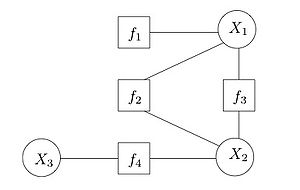
\includegraphics[width=6cm, height=3.5cm]{factor_graph}
	\end{center}
	\caption{A factor graph over three random variables and four factors which factorizes as $p(X) = \frac{1}{Z}f_1(x_1)f_2(x_1, x_2)f_3(x_1, x_2)f_4(x_2, x_3)$.}
\end{figure}

Another common PGM representation are factor graphs shown in Fig. 2.  A factor graph explicitly represents the factors functions $\psi_i$ which define the factorization of the joint probability distribution.  Later we will see that TensorLog converts atomic logical formula to a factor graph representation for differentiable logical inference.

In the remainder of this section we will introduce two popular algorithms for inference and learning in PGMs: Belief Propagation and Expectation Maximization.  We conclude with an introduction to Markov Logic Networks. 
\subsection{Belief Propagation}
In practice we will be interested in using a PGM to perform inference over some subset of the random variables; ie. computing the probability of the subset $p(X' \subseteq X)$.  We may have another subset $Y \subset X$, $X' \cap Y = \emptyset$ of observed variables in which case we wish to infer the conditional probability $p(X' | Y)$.

Fig. 3 ~\cite{Freeman13} shows a Markov chain with three observed variables $y_1, y_2, y_3$.  The factorization of this example is: 
\begin{gather}
p(X, Y) = \frac{1}{Z} \psi_{12}(x_1, x_2) \psi_{23}(x_2, x_3) \phi_1(x_1, y_1) \phi_2(x_2, y_2) \phi_3(x_3, y_3).
\end{gather}

Assume that we wish to compute the marginal probability of $x_1$ given $Y$: 
\begin{gather}
p(X_1 | Y) = \frac{1}{p(Y)} \sum_{X_2} \sum_{X_3} p(X, Y),
\end{gather}
where the equation is due to the fact that $p(X|Y) = \frac{p(X,Y)}{p(Y)}$.

Explicitly combining Eq. 1 and Eq. 2 and rearranging factors within summations simplifies to:
\begin{gather*}
p(X_1 | Y) = \frac{1}{p(Y)} \phi_1(X_1, y_1) \sum_{X_2 = x_2} \psi_{12}(X_1, x_2) \phi_2(x_2, y_2) \sum_{X_3 = x_3} \psi_{23}(x_2, x_3) \phi_3(x_3, y_3)\\
= \frac{1}{p(Y)} m_{41}(x_1) \sum_{X_2 = x_2} \psi_{12}(X_1, x_2) m_{52}(x_2) \sum_{X_3 = x_3} \psi_{23}(x_2, x_3) m_{63}(x_3)
\end{gather*}
We replace the $\phi_i(x_i, y_i)$ with a ``message" from $y_i$ to $x_i$.  The subscripts of the message correspond to the node numbering shown in Fig. 3 and $m_{ij}$ is the message from node $i$ to node $j$.  A message $m$ is a reusable partially marginalized probability vector, where the remaining marginalization required is over the receiver of the message.  For example, $Y_3$ ``says" to $X_3$ via $m_{63}(x_3)$ that if you provide some value $X_3 = x_3$ I will return the value of $x_3 | y_3$.

\begin{figure}
	\begin{center}
		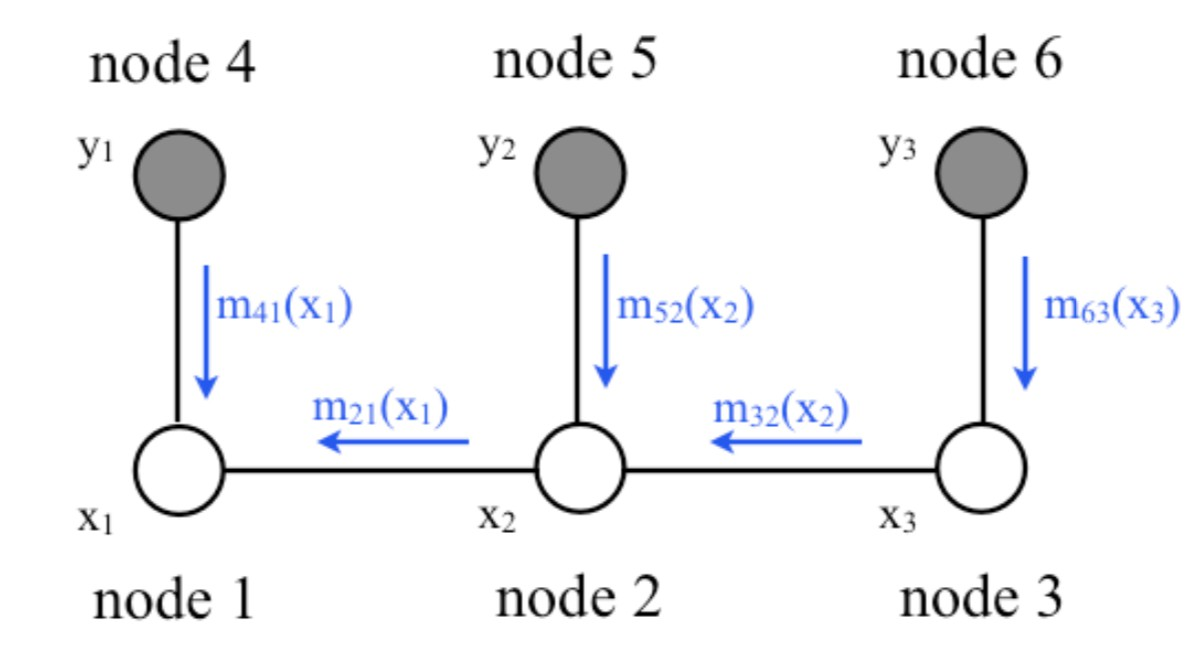
\includegraphics[width=8cm, height=4cm]{bp}
	\end{center}
	\caption{Markov chain with three observed variables $y_1, y_2, y_3$ and three hidden state variables $x_1, x_2, x_3$.  The arrows show the messages computed for $p(x_1 | Y)$.}
\end{figure}

Finishing the example above we find:
\begin{gather*}
p(X_1 | Y) = \frac{1}{p(Y)} m_{41}(x_1) \sum_{X_2 = x_2} \psi_{12}(X_1, x_2) m_{52}(x_2) \sum_{X_3 = x_3} \psi_{23}(x_2, x_3) m_{63}(x_3)\\
= \frac{1}{p(Y)} m_{41}(x_1) \sum_{X_2 = x_2} \psi_{12}(X_1, x_2) m_{52}(x_2) m_{32}(x_2)\\
= \frac{1}{p(Y)} m_{41}(x_1) m_{21}(x_1).
\end{gather*}

The Belief Propagation (BP) algorithm uses the idea of message passing to define a dynamic programming approach to the probabilistic inference problem.  If the PGM has no loops BP will return the exact probability for inference.  Even in the presence of cycles in the PGM many systems will still use (loopy) BP for inference.  BP for undirected graphical models is defined as follows:\\
1.  Convert the PGM to an equivalent PGM with only pairwise potentials.\\
2.  Compute $m_{ji}(x_i)$ as:
\begin{gather*}
m_{ji}(x_i) = \sum_{X_j = x_j} \psi_{ij}(x_i, x_j) \prod_{k \in N(j) \setminus i} m_{kj}(x_j),
\end{gather*}
where $N(j) \setminus i$ is the set of neighbors of node $x_j$ excluding $x_i$.  We may finally compute the marginal probability as $p(x_i) = \prod_{j} m_{ji}(x_i)$.  BP for factor graphs and directed graphical models follows a similar derivation but will not be explicitly derived in this report.

\subsection{Expectation Maximization}
In many applications we wish to learn the parameters $\boldsymbol{\theta}$ of a probability distribution $\mathcal{D}_{\boldsymbol{\theta}}$ using a dataset $\mathcal{X}$ which contains examples $x^{(i)} \sim \mathcal{D}_{\boldsymbol{\theta}}$.  As an example, we may be interested in determining the probability that a coin flip results in heads using an arbitrary coin and many i.i.d. repeated trials.

Generally there are three main approaches to parameter estimation: Maximum Likelihood (MLE), Maximum A Priori (MAP), and Bayesian estimation~\cite{Prince:2012:CVM:2344089}.  In the coin flipping example MLE would return $\theta = heads/flips$.  Formally this corresponds to maximizing the likelihood function $\mathcal{L}(\boldsymbol{\theta})$ with respect to the parameters:
\begin{gather*}
\argmax_{\boldsymbol{\theta}} \mathcal{L}(\boldsymbol{\theta})
= \argmax_{\boldsymbol{\theta}} p(\mathcal{X}|\boldsymbol{\theta})
= \argmax_{\boldsymbol{\theta}} \prod_i p(x^{(i)}|\boldsymbol{\theta})
= \argmax_{\boldsymbol{\theta}} \sum_i \log p(x^{(i)}|\boldsymbol{\theta})
\end{gather*}
the last equality maximizes the log-likelihood and has the same maximizing $\boldsymbol{\theta}$ as $\mathcal{L}(\boldsymbol{\theta})$ since the log function is monotonically increasing.

The Expectation Maximization (EM) algorithm is a generalization of MLE to the case where we have unobserved hidden variables $z$ and wish to learn the parameters for $p(\mathcal{X}, Z)$~\cite{Ng}.  Attempting MLE on this joint distribution gives:
\begin{gather*}
MLE(\mathcal{X}) = \argmax_{\boldsymbol{\theta}} \sum_i \log  \sum_{z^{(i)}}  p(x^{(i)}, z^{(i)}|\boldsymbol{\theta}),
\end{gather*}
where we marginalize on $z$ since our data only contains $x$.  In general this maximization may not be tractable due to the marginalization over $z$.

The EM algorithm circumvents this intractable marginalization by rewriting the log-likelihood function using Jensen's Inequality: $\mathbf{E}[f(X)] \leq f(\mathbf{E}[X])$ when $f$ is a concave function and $X$ is a random variable.  If $f$ is strictly concave then $\mathbf{E}[f(X)] = f(\mathbf{E}[X])$ iff $X = \mathbf{E}[X]$.  This last condition is satisfied when $X$ is a constant. 

Using Jensen's Inequality we derive:
\begin{gather}
\log \mathcal{L}(\boldsymbol{\theta}) = \sum_i \log \sum_{z^{(i)}} p(x^{(i)}, z^{(i)}|\boldsymbol{\theta})\nonumber \\
= \sum_i \log \sum_{z^{(i)}} Q_i(z^{(i)}) \frac{p(x^{(i)}, z^{(i)}|\boldsymbol{\theta})}{Q_i(z^{(i)})} \nonumber \\
\geq \sum_i \sum_{z^{(i)}} Q_i(z^{(i)})  \log \frac{p(x^{(i)}, z^{(i)}|\boldsymbol{\theta})}{Q_i(z^{(i)})},
\end{gather}
where $Q_i(z^{(i)})$ is some arbitrary distribution over $z^{(i)}$.  Jensen's Inequality holds since $f$ is the log function which is strictly concave and the expectation is with respect to $z^{(i)} \sim Q_i$.

The key observation is that the inequality in Eq. 3 holds for any distribution $Q_i$ given some $\boldsymbol{\theta}$.  To find the $Q_i$ which maximizes Eq. 3 (ie. makes the inequality an equality) we will use the fact that $\mathbf{E}[f(X)] = f(\mathbf{E}[X])$ when $X$ is a constant.  Let $Q_i(z^{(i)}) \propto p(x^{(i)}, z^{(i)}|\boldsymbol{\theta})$.  Then:
\begin{gather*}
\frac{p(x^{(i)}, z^{(i)}|\boldsymbol{\theta})}{Q_i(z^{(i)})} = \frac{p(x^{(i)}, z^{(i)}|\boldsymbol{\theta})}{ p(x^{(i)}, z^{(i)}|\boldsymbol{\theta}) \cdot \alpha} = \frac{1}{\alpha}.
\end{gather*}
Given the fact that $Q_i$ is a distribution we know that if $Q_i(z^{(i)}) \propto p(x^{(i)}, z^{(i)}|\boldsymbol{\theta})$ then the constant $\alpha = \frac{1}{Z}$ where $Z = \sum_z p(x^{(i)}, z^{(i)}|\boldsymbol{\theta})$.  So in fact: 
\begin{gather*}
Q_i(z^{(i)}) = \frac{p(x^{(i)}, z^{(i)}|\boldsymbol{\theta})}{\sum_z p(x^{(i)}, z^{(i)}|\boldsymbol{\theta})} = \frac{p(x^{(i)}, z^{(i)}|\boldsymbol{\theta})}{p(x^{(i)}|\boldsymbol{\theta})} = p(z^{(i)} | x^{(i)}; \boldsymbol{\theta}).
\end{gather*}
\begin{mdframed}[linewidth=.8pt]
	\begin{algorithm}[H]
		\KwData{
			Training data $\mathcal{X} = \{\textbf{x}^{(n)}\}_{n = 1}^{N}$
		}
		\KwResult{$\boldsymbol{\theta}^*$ which maximizes $\mathcal{L}(\boldsymbol{\theta})$\newline}
		Initialize model parameters $\boldsymbol{\theta}$ \\
		\While{$\lnot$ converged}{
			\For{$x^{(i)} \in \mathcal{X}$}{ (E-step) 
				$Q_i(z^{(i)}) \leftarrow p(z^{(i)} | x^{(i)}; \boldsymbol{\theta})$
			}
			
			(M-step) $\boldsymbol{\theta} \leftarrow \argmax_{\boldsymbol{\theta}} \sum_i \sum_{z^{(i)}} Q_i(z^{(i)}) \log \frac{p(x^{(i)}, z^{(i)}| \boldsymbol{\theta})}{Q_i(z^{(i)})}$
		}
		\caption{Expectation Maximization}
	\end{algorithm}
\end{mdframed}

The final EM algorithm is presented in Algorithm 1.  We can view the EM algorithm as alternatively optimizing the lower bound given in Eq. 3 (E-step) and optimizing the parameters of the model (M-step).  Note that the E-step is critical so that when we optimize $\boldsymbol{\theta}$ we are in fact maximizing the log-likelihood (with respect to the current estimates of $\boldsymbol{\theta}$).

\subsection{Case Study: Markov Logic Networks}
Markov Logic Networks (MLN) provide a framework for combing logical knowledge bases and PGMs~\cite{Richardson:2006:MLN:1113907.1113910}.  An MLN is a first-order knowledge base of weighted formulas which are used to construct Markov networks.  Formally, a MLN $L$ is a set of pairs $(F_i, w_i)$ where $F_i$ is a first-order logic formula over a finite domain $C = \{c_1, ..., c_{|C|}\}$ and $w_i \in \mathbf{R}$.  

MLNs follow a possible worlds semantics where the probability that some $F_i$ is true is a function of probabilities of the possible worlds in which the formula is true.  A possible world is a domain ($D$), a set of functions ($f: D \times ... \times D \rightarrow D$), a set of relations (which correspond to predicates), and an interpretation which maps symbols from $L$ and $C$ to $D$.

The constructed Markov network $M_{L, C}$ contains one binary node for each possible grounding of each predicate in $L$ which takes the value 1 if the ground atom is true, and 0 otherwise.  $M_{L, C}$ contains one feature for each grounding of each formula $F_i \in L$ where the value of the feature is 1 if the formula is true, and 0 otherwise. The weight of the feature for $F_i$ is $w_i$.

Given a set of constants $C$ the MLN will define a different ground Markov network.  The probability over possible worlds $X = x$ specified by the ground MLN $M_{L, C}$ is:
\begin{gather*}
p(X = x | M_{L, C}) = \frac{1}{Z} \prod_i \phi_i(x_{\{i\}})^{n_i(x)} =  \frac{1}{Z} \exp \bigg( \sum_i w_i n_i(x) \bigg)
\end{gather*}
where $n_i(x)$ is the number of true groundings of $F_i$ in $x$ and $x_{\{i\}}$ is the truth values of the atoms appearing in $F_i$.

\begin{figure}
	\begin{center}
		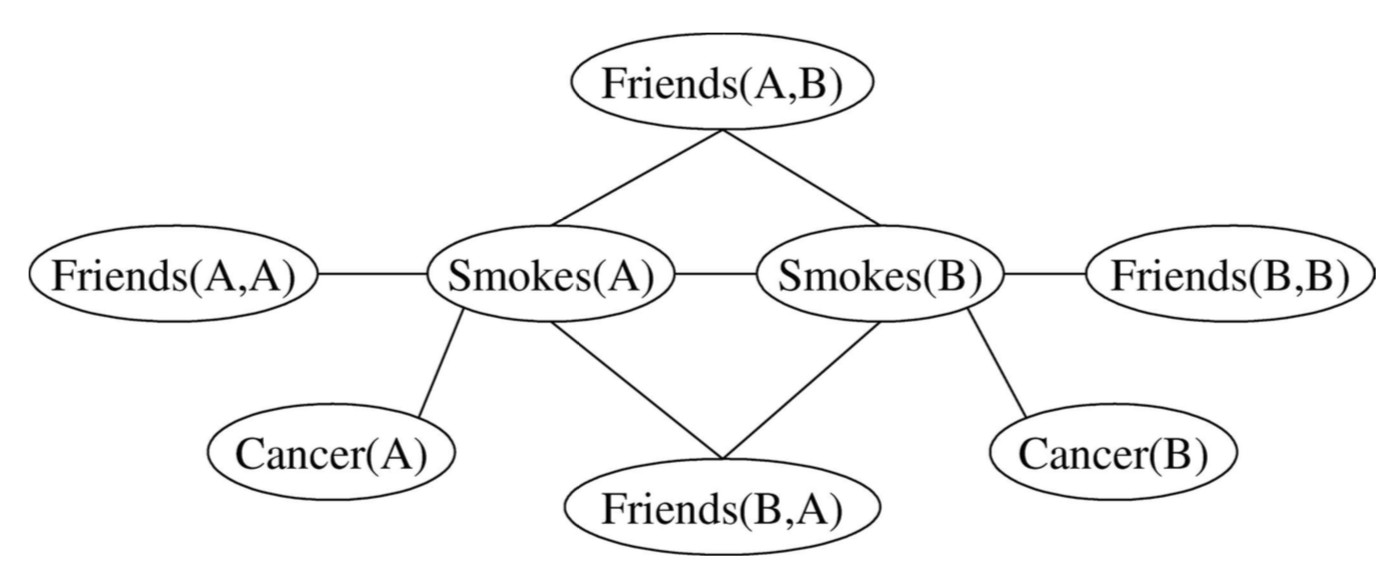
\includegraphics[width=8cm, height=3.5cm]{mln}
	\end{center}
	\caption{Ground MLN over $C = \{A, B\}$}
\end{figure}
Fig. 4~\cite{Richardson:2006:MLN:1113907.1113910} shows a ground MLN with constants $C = \{A, B\}$ and weighted formulas:
\begin{gather*}
1.5 :: \forall x Smokes(x) \Rightarrow Cancer(x) \\
1.1 :: \forall x \forall y Friends(x, y) \Rightarrow (Smokes(x) \Leftrightarrow Smokes(y))
\end{gather*} 

Each possible world over $L$ defines the truth value of each node in $M_{L, C}$ which in turn defines the probability of the possible world.  Having formalized the correspondence between weighted logic formulas and PGMs we may now use standard PGM inference methods (such as MCMC or Lifted BP) to determine the probability of that a logical formula is true.  For example the probability that two formulas $F_1$ and $F_2$ hold can be computed as:
\begin{gather*}
p(F_1 \land F_2 | M_{L, C}) = \sum_{x \in X_{F_1} \cap X_{F_2}} p(X=x | M_{L, C}),
\end{gather*}
where $X_{F_i}$ is the set of worlds in which $F_i$ holds.

\section{Probabilistic Logic Programming}
Many languages have been proposed for PLP including PRISM~\cite{Sato:1997:PLS:1622270.1622348}, ProbLog~\cite{DeRaedt:2007:PPP:1625275.1625673}, and Stochastic Logic Programs~\cite{Muggleton96stochasticlogic}.  While there are differences in the language implementations, these probabilistic Prologs share a common theoretical basis in the distribution semantics~\cite{Sato95astatistical}.  The distribution semantics extends the least model semantics of Prolog to handle possible worlds which are weighted by the likelihood of the set of true facts in the particular world.  

In Section 2.1 we formalize the distribution semantics and provide examples of PLP programs.  Section 2.2 is concerned with inference techniques in traditional PLP systems, which will be contrasted by the differentiable process proposed in the TensorLog system later in this report.  We conclude our treatment of PLP with an introduction to parameter learning in PRISM.

\subsection{Distribution Semantics}
\begin{figure}
	\begin{verbatim}
	% Rules
	call :- calls(X).
	calls(X) :- alarm, hears_alarm(X).
	alarm :- earthquake; burglary.
	
	% Facts
	0.7::hears_alarm(john).
	0.4::hears_alarm(mary).
	0.1::burglary.
	0.2::earthquake.
	\end{verbatim}
	\caption{ProbLog program for the alarm world.}
\end{figure}
A PLP program $P$ can be partitioned as $P = F \cup R$ where $F$ is the set of probabilistic facts and $R$ is the set of rules.  The rule set $R$ is held fixed while possible worlds are considered with respect to the possible subsets of $F$.  A possible world is some $F' \subseteq F$, where all $f_i \in F'$ are true, along with all facts derivable from $F' \cup R$.  We also assume the closed world assumption with respect to the probability computations~\cite{Getoor:2007:ISR:1296231}.

A typical ProbLog program is shown in Fig. 6 which models the well known alarm world Bayesian network~\cite{DeRaedt:2015:PPC:2812521.2812529}.  In ProbLog's notation, a binary random variable is defined as $\theta::X$ where $p(X = True) = \theta$ and $p(X = False) = 1 - \theta$.

In general we are interested in the probability of a query $p(\mathbf{q})$.  For example we may wish to infer the probability of a call given the program: $p(call| P)$.  A query probability can be computed by summation over probabilities of the possible worlds which entail the query.  

The probability of $F'$ (denoted $P_F$) is computed as:
\begin{gather}
P_F(F') = \prod_{f_i \in F'} \theta_i \times \prod_{f_i \in F \setminus F'} 1 - \theta_i.
\end{gather} 
Thus we can compute $p(\mathbf{q})$ as:
\begin{equation}
\begin{gathered}
p(\mathbf{q}) = \sum_{F' : \exists \sigma F' \cup R \models \mathbf{q}\sigma} P_F(F')\\
= \sum_{F':\exists \sigma F' \cup R \models \mathbf{q}\sigma} \prod_{f_i \in F'} \theta_i \times \prod_{f_i \in F \setminus F'} 1 - \theta_i,
\end{gathered}
\end{equation}
where $\sigma$ is a logical substitution.

The preceding treatment only considered binary random variables which were sampled exactly once.  One modification is that we allow random processes $X$ which may be sampled many times in the execution of a program.  We make the standard i.i.d. assumption with respect to each $x_i \sim X$.  

\begin{figure}
	\begin{verbatim}
	% Rules
	call :- calls(X).
	calls(X) :- alarm, msw(hears_alarm(X), true).
	alarm :- msw(earthquake, true); msw(burglary, true).
	
	% msw definitions
	values(hears_alarm(john), [true, busy, false], [0.7, 0.1, 0.2]).
	values(hears_alarm(mary), [true, busy, false], [0.4, 0.4, 0.2]).
	values(burglary, [true, false], [0.1, 0.9]).
	values(earthquake, [true, false], [0.2, 0.8]).
	\end{verbatim}
	\caption{PRISM program for the alarm world.}
\end{figure}

A second extension that is commonly adopted in PLP languages is assuming the probabilistic facts are drawn i.i.d. from a categorical distribution.  This is the convention that PRISM adopts with the \verb!msw/3! notation.  In PRISM an \verb!msw!$(X, I, O)$ predicate has the interpretation that $X$ is some random process, $I$ is the i.i.d. instance number of the current trial, and $O$ is the outcome of the current trial.  Fig. 6 shows the alarm world example implemented as a PRISM program.  In this program the neighbors may hear the alarm yet be too busy to call you, but otherwise follows the same logic as Fig. 5.  To extend Eq. 4 to handle the categorical case, simply replace $\theta_i$ with $p(X_I = O)$.

\subsection{Inference}
While PLPs are similar to MLNs in the fact that they both follow a possible worlds semantics, standard inference methods implemented in PLPs need not use any inference techniques over a PGM.

The inference task we will consider for this report is that of computing the likelihood of a query $p(\mathbf{q})$.  There are other inference tasks which are possible in a PLP system such as Viterbi, marginal, and MAP inference but the algorithms and techniques are not within the scope of this report~\cite{DeRaedt:2015:PPC:2812521.2812529}.

Similarly to Prolog, we can attempt to compute $p(\mathbf{q})$ in a bottom up (forward reasoning) or top down (backward reasoning) manner.  The naive algorithm simply iterates through all $F' \subseteq F$ and computes Eq. 5 using either the forward or backward reasoning procedure.

Backward reasoning is the SLD-resolution algorithm.  The SLD-resolution algorithm works via the principle of resolution:
\begin{gather*}
A \lor B \land \neg A \lor C \equiv B \lor C.
\end{gather*}  
We formalize the query as \verb!:-! $\mathbf{q}$, which is equivalent to $\neg \mathbf{q}$, and proceed using the principle of resolution until we reach the special \verb!ff! symbol.

The proof for $calls(john)$ when $F' = \{alarm, hears\_alarm(john) \}$ is:
\begin{verbatim}
                                calls(john)
                                |  calls(X) :- alarm, hears_alarm(X).
                                alarm, hears_alarm(john).
                                |  alarm
                                hears_alarm(john).
                                |  hears_alarm(john).
                                ff
\end{verbatim}
In general the set of all proofs for a query will form a tree which may also have failed and possibly infinite derivations.  We only compute the probability of those $F'$ which model $\mathbf{q}$.

The bottom up construction uses the $T_P$ operator to iteratively build the set of facts derivable in $F' \cup R$.  Using the program of Fig. 6 and taking $F' = \{ burglary \}$ forward reasoning proceeds as follows:
\begin{gather*}
T_P(F') = \{ burglary \} \\
T_P^2(F') = \{ burglary, alarm \} \\
T_P^3(F') = \{ burglary, alarm \} = T_P^2(F').
\end{gather*}
For our inference task we would only keep the probabilities for those $F'$ in which $F' \cup R \models \mathbf{q}$.

\subsection{Learning}
PRISM implements many standard parameter learning algorithms such as the EM and Variational EM algorithms~\cite{prism}.  Using the observation that a PLP program is parameterized by the probabilities of $F$, PRISM uses these algorithms to fit the parameters of a program using a dataset in the form of a collection of ground clauses.

Returning to the alarm world example in Fig. 6 the dataset would be a collection of queries such as $\{ call, \neg call, \neg call, \neg call, call\}$.  Given that a call may occur under many different $F'$ we are in a partially observing state and will use the EM algorithm to learn the parameters of $P$.  If we were in a situation which was fully observable (Ex: John is your only neighbor and earthquakes are the only trigger for your alarm) PRISM will learn the parameters of $P$ using MLE.

More formally, if the dataset was a collection of goals (with the same predicate and arity) $G_i$ of the form $\{G_1, ..., G_m\}$ then MLE will fit the parameters $\theta_o$ of \verb!msw!$(X, I, O)$ as $\theta_o = C_{x, o} / \sum_{o'} C_{x, o'}$ where $C_{x, o}$ is the number of times $O = o$ for switch $X = x$.  The partially observable case proceeds in a similar manner but computes the expectation that $O = o$ under parameters $\theta^{t}$ in the E-step and obtains $\theta^{t + 1}$ using the same counting argument as in MLE for the M-step.

\subsection{Case Study: LOHMM Parameter Fitting in PRISM}
Hidden Markov Models (HMM) are a directed probabilistic graphical model for discrete temporal sequences of observed random variables $O$, along with the hidden states $X$ which caused the observations.  The joint probability of an HMM factorizes as:
\begin{gather*}
p(X, O) = \prod_t p(o_t | x_t) \times \prod_t p(x_t | x_{t - 1}).
\end{gather*}

HMMs have two sets of parameters: those which govern the emission probability conditioned on the current hidden state, and the transition probabilities which determine $p(x_t | x_{t - 1})$.

Logical Hidden Markov Models (LOHMM)~\cite{Kersting06logicalhidden} are a generalization of the HMM to a first-order representation which uses abstract transitions to define a first-order PGM.  An abstract transition is defined as $p: H \xleftarrow{O} B$ where $p$ is the probability of the transition and $H, B, O$ are first-order atoms.  
As an example:
\begin{gather*}
0.8 : xdvi(File, dvi) \xleftarrow{latex(File)} latex(File, tex)
\end{gather*}
defines an abstract transition where starting the state $latex(File, tex)$ the LOHMM transitions to the state $xdvi(File, dvi)$ and emits the observation $latex(File)$.  Here $File$ is not ground and would be determined via unification.

The definition of an abstract transition combines the transition and emission probabilities of a standard HMM.  LOHMMs introduce a set of parameters $\boldsymbol{\mu}$ which governs the distribution of grounding a first-order abstract transition.  This is the main difference in parameterization between LOHMMs and HMMs.  The introduction of $\boldsymbol{\mu}$ changes the necessary inference and learning algorithms for HMMs.  Kersting et al.~\cite{Kersting06logicalhidden} presented an extension to the standard algorithms for HMMs to handle the LOHMM case.  While this extension is very natural and aesthetically similar to the HMM case, designing and implementing a novel algorithm for LOHMMs surely was not a trivial task.

Defining either HMMs or LOHMMs in a PLP is straightforward.  In particular we encoded the LOHMM model as a PRISM program.  After having defined the required distributions as \verb!msw! atoms along with the general program logic, the parameter learning and inference procedures native to PRISM computed the required functionality.  Thus our encoding is capable of learning the distribution of the parameters in an LOHMM and is similarly able to infer the probability of some query without the need to explicitly introduce novel algorithms.

\section{Deep Learning}

\begin{figure}
	\begin{center}
		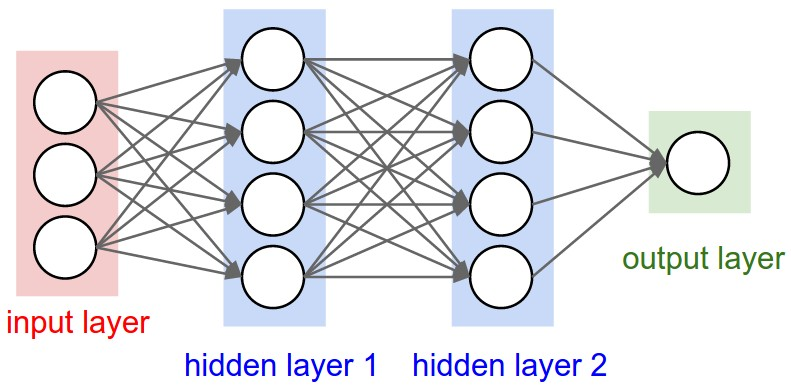
\includegraphics[width=8cm, height=4cm]{dnn}
	\end{center}
	\caption{A two layer neural network.}
\end{figure}
The field of deep learning is focused on a class of learning algorithms called Deep Neural Networks (DNN).  A DNN is a collection of neurons which learns a nonlinear function over the input data.  Fig. 7 shows a typical feed forward neural network with fully connected layers.  Each node in a hidden layer will define a non-linear function of the node's input.  Typically this is some function $\phi(\textbf{w}^{\top} \textbf{x} + b)$ where $\textbf{x}$ is the input vector to the node, $\textbf{w}$ and $b$ are parameters, and $\phi$ is typically a nonlinear function such as the logistic sigmoid.  Since a hidden layer node will provide it's output as input to each node in the next layer, one can interpret a DNN as learning higher level features as computation proceeds to the output layer.

DNNs are appropriate for all learning settings, however we will mainly consider supervised learning in this report.  In the supervised learning setting we have a training set $\mathcal{S} = (\mathcal{X}, \mathcal{Y}) = \{ \textbf{x}^{(i)}, \textbf{y}^{(i)} \}_{i = 1}^{m}$ of $m$ training instances where $\textbf{x}^{(i)}$ is the $ith$ data point and $\textbf{y}^{(i)}$ is the associated ground truth vector.  In a DNN the elements of $\textbf{x}^{(i)}$ populate the input layer neurons while the output layer has the same dimensionality as $\textbf{y}^{(i)}$.  The goal of supervised learning is to learn the parameters of a function $ f_{\boldsymbol{\theta}}: \mathcal{X} \rightarrow \mathcal{Y}  $ which is parameterized by $ \boldsymbol{\theta} $.  Typically we introduce a loss function $\mathcal{L}(\mathcal{S} ;\boldsymbol{\theta})$ which is defined over $\mathcal{S}$ and $f$.  For example, a typical loss used for regression is the mean squared error: 

\begin{gather*}
\mathcal{L}_{\text{mse}}(\mathcal{S} ;\boldsymbol{\theta}) = \frac{1}{m} \sum_{i = 1}^{m} (\textbf{y}^{(i)} - \hat{\textbf{y}}^{(i)})^2
\end{gather*}
where $f_{\boldsymbol{\theta}}(\textbf{x}^{(i)}) = \hat{\textbf{y}}^{(i)}$.

Depending on the specific problem setting a DNN may apply some function $\psi(\textbf{y})$ to the output layer's output.  In this report we will be mostly concerned with multiclass classification problems where it is common for $\psi$ to be the softmax function:
\begin{gather*}
softmax(y_i) = \frac{e^{y_i}}{\sum_{j = 1}^{k} e^{y_j}}.
\end{gather*}
For DNNs the softmax function operates on the output layer's computed vector and returns a probability vector $\boldsymbol{\sigma}$ which has the interpretation that $\sigma_k = p(y^{(i)} = k | \textbf{x}^{(i)})$; the probability that the current example $\textbf{x}^{(i)}$ is of class $k$.  

The standard loss function for multiclass classification is the cross-entropy loss:
\begin{gather*}
\mathcal{L}_{cross-entropy}( \textbf{y}, \hat{\textbf{y}}) = - \sum_{i} y_i \log(\hat{y}_i)
\end{gather*}
which represents the difference in probability distributions of the target distribution $\mathcal{P}(y)$ and the estimated distribution $\mathcal{Q}(\hat{y})$.

\begin{mdframed}[linewidth=.8pt]
	\begin{algorithm}[H]
		\KwData{
			Training data $\mathcal{S} = \{(\textbf{x}^{(n)}, \textbf{y}^{(n)})\}_{n = 1}^{N}$,\\
			\hspace*{1.15cm} Hyperparameters: $\eta$ learning rate
		}
		\KwResult{$\boldsymbol{\theta}^*$ which minimizes $\mathcal{L}$\newline}
		Initialize DNN parameters $\boldsymbol{\theta}$ \\
		\While{$\lnot$ converged}{
			Sample a minibatch $(X, Y) \subset \mathcal{S}$ \\
			Set $g \leftarrow 0$ \\
			\For{$(\textbf{x}, \textbf{y}) \in (X, Y)$}{
				Compute gradient: $g \leftarrow g + \nabla_\theta \mathcal{L}(f_\theta(\textbf{x}), \textbf{y}; \boldsymbol{\theta})$
			}
			Apply update: $\boldsymbol{\theta} \leftarrow \boldsymbol{\theta} - \eta g$
		}
		\caption{Stochastic Gradient Descent}
	\end{algorithm}
\end{mdframed}

Having defined a suitable function $f$ and loss $\mathcal{L}$ we attempt to minimize the loss function.  There are many possible ways to attempt this optimization.  In the context of deep learning we typically use the Stochastic Gradient Descent (SGD) algorithm where the parameter gradients of the complex nested function defined by the neural network are computed using the backpropagation algorithm.  The backpropagation algorithm is simply recursive application of the chain rule of calculus.  The SGD algorithm is shown in Algorithm 2.  Starting from the loss we compute $\nabla_{\boldsymbol{\theta}} \mathcal{L}(\mathcal{S} ;\boldsymbol{\theta})$ using backpropagation where $\nabla_{\boldsymbol{\theta}i} = \frac{\partial \mathcal{L}}{\partial \theta_i }$ is the gradient vector.  Having computed these partial derivatives we use SGD to update the parameters $\boldsymbol{\hat{\theta}} \leftarrow \boldsymbol{\theta} - \eta \sum_{i \in B} \nabla_{\boldsymbol{\theta}} \mathcal{L}(f(\textbf{x}^{(i)}), \textbf{y}^{(i)} ;\boldsymbol{\theta})$ where $\eta$ is the learning rate and $B$ is the minibatch.

\subsection{DNN Architectures}
There are many extensions to the basic feed forward DNN shown in Fig. 7.  Some of the most popular include convolutional neural networks (CNN) and recurrent neural networks (RNN).  Both CNNs and RNNs reduce the number of parameters of the network via parameter sharing.  A standard fully connected feed forward DNN will have $nm$ weights per hidden layer, ignoring the bias terms.  In the case of a CNN the filter weights of the learned convolutions are shared across the input volume.  RNNs operate over temporal data and achieve parameter reduction by reusing the same weight matrices over each time step.  

One other well known DNN architecture is the class of autoencoders.  Shown in Fig. 8 an autoencoder is a network which learns a low dimensional feature representation of the input space using an encoder and decoder architecture.  The encoder network maps an input vector to a lower dimensional fully connected hidden layer.  The decoder then uses this lower dimensional hidden layer as it's input vector and tries to recreate the original vector.  The autoencoder network is trained using unsupervised learning where the loss is typically the mean squared error over the original input and the reconstructed output: 
\begin{gather*}
\frac{1}{m} \sum_{i = 1}^{m} (\textbf{x}^{(i)} - \hat{\textbf{x}}^{(i)})^2.
\end{gather*}
\begin{figure}
	\begin{center}
		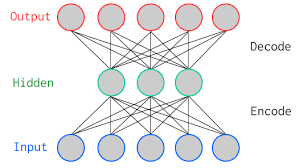
\includegraphics[height=4cm, width=7cm]{autoencoder}
	\end{center}
	\caption{An autoencoder network.}
\end{figure}

\subsection{Case Study: Word Embeddings}
Later in this report we will use the sentiment analysis problem as an example showcasing the capacity of logical regularization rules in training a DNN.  In this example the subject of word embeddings play a central part in understanding the architecture of the neural network.  Word embeddings are an interesting subject in their own right and have been a hot topic in natural language processing (NLP) and machine learning for the past decade.

Traditionally in NLP a word from some vocabulary $V$ is represented as a one-hot vector $\textbf{w} \in \mathbf{R}^{|V|}$.  $\textbf{w}$ can be thought of as an array where the indices correspond to specific vocabulary words and only a single index has a value of $1$ while all other entries have a value of $0$.  A collection of $m$ words, or a document, would then be represented as $\textbf{d} = \sum_{i=1}^{m} \textbf{w}^{(i)}$.  This is the well known bag of words feature representation scheme.

Even for large documents the entries of $\textbf{d}$ will tend to be sparse given a rich enough vocabulary.  While sparsity presents a troubling issue, there is another more fundamental problem with the one-hot vector approach.  One-hot vectors have no semantic interpretation.  The vector for ``dog" and the vector for ``cat" may be one index apart or have indices at opposite ends of the vector.  However both concepts share many characteristics.

Word embeddings use deep learning to learn a semantically meaningful dense vector representation of a vocabulary.  The main idea is to use large corpora of unlabeled natural language to train a variation of an autoencoder network.

The input vector to the autoencoder network will be a one-hot vector representation of a word, $\textbf{w} \in \mathbf{R}^{|V|}$, which is fed to a fully connected layer with $k$ hidden units with weight matrix $\mathcal{T} \in \mathcal{R}^{|V| \times k}$.  Since the hidden layer computes $\textbf{w}_i^{\top} \mathcal{T} = \textbf{h}_i$ using a one-hot vector, only the weights corresponding to the $ith$ word will have any consequence.  In fact, the $jth$ element of $\textbf{h}_i$ is exactly the $ith$ weight to the $jth$ hidden unit.  For this reason, $\mathcal{T}$ can be thought of as a lookup table and $\textbf{h}$ is the dense vector representation of $\textbf{w}$.

The network will  output a softmax vector $\boldsymbol{\sigma}_\theta \in \mathbf{R}^{|V|}$.  The $ith$ element of $\boldsymbol{\sigma}_\theta$ corresponds to the likelihood that the $ith$ vocabulary word would be within a window of $k$ words around the input word.  This $k$ width window is called the context of a word and the network is trained in an unsupervised manner using contexts of words taken from sentences of the corpora.  For example: ``the black \textbf{dog} ate food" has four context pairs for learning 
\begin{gather*}
\{ (dog, the), (dog, black), (dog, ate), (dog, food) \}.
\end{gather*}
If we were to replace ``dog" with ``cat" or ``horse" the sentence would still be meaningful.  On the other hand replacing ``dog" with ``house" is nonsense.  By randomly replacing the correct word with another word in the vocabulary we can generate negative examples as well.  The choice of loss function varies depending on the architecture (Word2Vec~\cite{Mikolov:2013:DRW:2999792.2999959}, GloVe~\cite{Pennington14glove:global}, etc), and is will not be discussed in this report.  

Since similar words appear in similar contexts, the training of the network will learn similar vector weights for similar words.  This will in turn give a semantically meaningful representation of the vocabulary.  After training the network we only save $\mathcal{T}$ and can reuse this lookup table as a feature set for other tasks.
 
\section{Deep Neural Networks with Logic Rules}

Hu et al.~\cite{Hu2016HarnessingDN} propose a framework for incorporating expert knowledge in the form of logic rules within arbitrary deep neural networks.  Fig. 9 shows the abstract network architecture which is composed of student and teacher networks.
\begin{figure}
	\begin{center}
		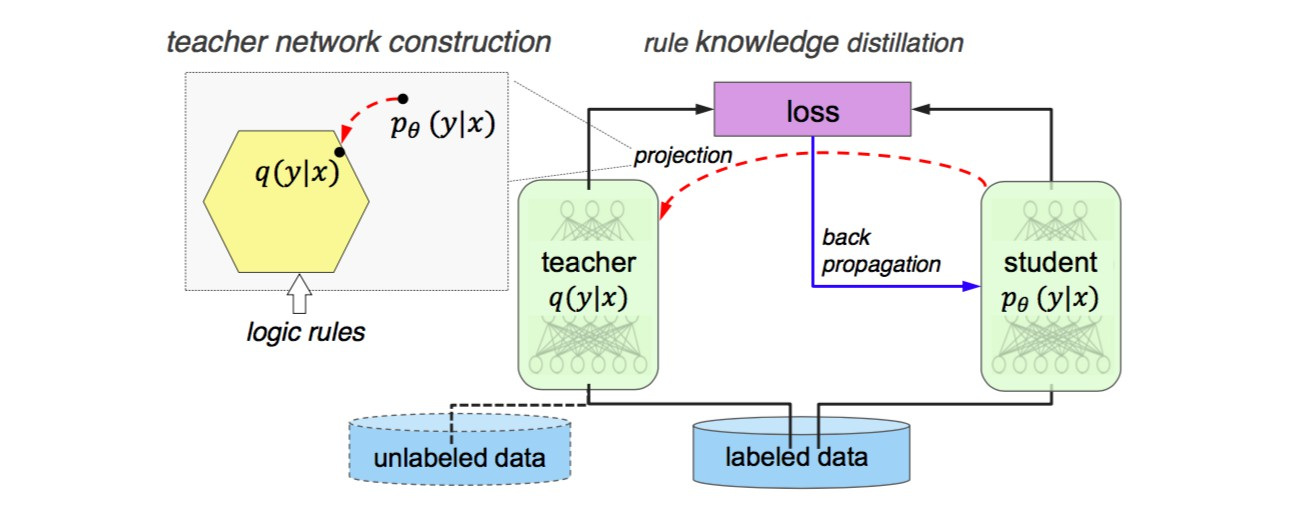
\includegraphics[width=12cm, height=5cm]{teacher_dnn}
	\end{center}
	\caption{The augmented DNN is a teacher and student network optimizing a dual objective.}
\end{figure}
The teacher network $q(y|x)$ is constructed by a ``projection" from the student network $p_\theta(y|x)$.  This projection function is realized by optimizing a dual criteria of approximating the student network output while satisfying the logical constraints.  The student network is a standard DNN such as a CNN which is optimizing a dual objective:
\begin{gather}
\boldsymbol{\theta}^{(t + 1)} = \argmin_{\theta \in \Theta} \frac{1}{N} \sum_{n = 1}^{N} (1 - \pi) \mathcal{L}(\textbf{y}_n, \boldsymbol{\sigma}_{\theta}(\textbf{x}_{n})) + \pi \mathcal{L}(s_n^{(t)}, \boldsymbol{\sigma}_{\theta}(\textbf{x}_n)).
\end{gather}
Here $\pi$ is the relative weighting of the loss components where $\mathcal{L}(\textbf{y}_n, \boldsymbol{\sigma}_{\theta}(\textbf{x}_{n}))$ represents the standard loss incurred by the DNN on the $nth$ example.  $\mathcal{L}(s_n^{(t)}, \boldsymbol{\sigma}_{\theta}(\textbf{x}_n))$ is the loss introduced by $q(y|x) = s_n^{(t)}$: the teacher network output from the current iteration.  By optimizing $\boldsymbol{\theta}$ with respect to $\mathcal{L}(s_n^{(t)}, \boldsymbol{\sigma}_{\theta}(\textbf{x}_n))$  the parameters of the student network will align with the logic rules embedded in the teacher network.

The loss function $\mathcal{L}$ can be any appropriate objective for the problem domain such as the cross-entropy loss and is of the same functional form for both loss components.  We will only consider the multiclass classification domain for this report and assume that the output is passed through a softmax activation function yielding the prediction vector $p_\theta(y|x) = \boldsymbol{\sigma}_{\theta}(\textbf{x}_{n})$.

\subsection{Logic Rules}
The logic rules of the teacher network are represented as a set $\mathcal{R} = \{(R_l, \lambda_l) \}_{l = 1}^L$ where each $R_l$ is a first-order logic formula with an associated confidence $\lambda_l \in [0, \infty]$.  A confidence level of $\lambda_l = \infty$ represents a hard rule where all groundings of $R_l$ must be true.  The set of groundings of $R_l$ is denoted as $\{ r_{lg}(X, Y) \}_{g=1}^{G_l}$ where $(X, Y) \subset (\mathcal{X}, \mathcal{Y})$.  The domain of a logical variable may be any subset of $\mathcal{X} \cup \mathcal{Y}$.

In this architecture logic rules serve as a sort of regularization over the possible models the DNN can assume.  These rules are encoded using a continuous logic called soft logic~\cite{2015arXiv150504406B} which allows continuous truth values $\in [0, 1]$.  The standard Boolean operators are redefined as:
\begin{equation}
\begin{gathered}
\neg A = 1 - A\\
A \& B = \max\{A + B - 1, 0\}\\
A \lor B = \min\{A + B, 1\}\\
A_1 \land ... \land A_N = \sum_i A_i / N
\end{gathered}
\end{equation}

These rules have an intuitive semantics when compared to the standard boolean operators.  For example $A \& B = B$ when $A = 1$, while $A \land B = B$ when $A = \top$ in classical propositional logic.  In soft logic $\land$ is defined as an averaging operation while $\&$ represents conjunction.  By adopting the semantics of soft logic the corresponding truth values of our logical formulas will be continuous and gradients will be computable in the learning phase.

\subsection{Teacher Network Construction}
The teacher network is constructed by optimizing a dual objective function with respect to the output of the student network:
\begin{equation}
\begin{gathered}
\min_{q, \xi \geq 0}  \text{KL}(q(Y|X) || p_\theta(Y|X)) + C \sum_{l, g_l} \xi_{l, g_l}\\
\text{s.t. } \lambda_l (1 - \mathbf{E}_q[r_{l,g_l}(X, Y)]) \leq \xi_{l, g_l}\\
g_l = 1,...,G_l, l= 1,..., L.
\end{gathered}
\end{equation}
The first criteria is optimizing the Kullback-Leibler divergence between $q(y|x)$ and $p_\theta(y|x)$ which represents a measure of similarity between the two distributions with respect to entropy.  The second criteria is formalized using an expectation operator over the groundings of the rules such that $\mathbf{E}_q[r_{l,g_l}(X, Y)] = 1$, which can be seen in the constraints.  This expectation is weighted by $\lambda_l$ and slack variables $\xi_{l, g_l}$ are introduced.  We solve this constrained optimization problem by solving the dual Lagrangian.

The dual Lagrangian is derived by explicitly considering all constraints in standard form:
\begin{gather*}
\min_{q, \xi} \text{KL}(q(Y|X) || p_\theta(Y|X)) + C \sum_{l, g_l} \xi_{l, g_l}\\
\text{s.t. } \lambda_l (1 - \mathbf{E}_q[r_{l,g_l}(X, Y)]) - \xi_{l, g_l}\leq 0\\
-\xi_{l, g_l} \leq 0\\
\sum_Y q(Y|X) - 1 = 0\\
g_l = 1,...,G_l, l= 1,..., L
\end{gather*}
and then introducing Lagrange multipliers where appropriate:
\begin{gather*}
\max_{\eta \geq 0, \mu \geq 0, \alpha \geq 0} \min_{q, \xi}  \text{KL}(q(Y|X) || p_\theta(Y|X)) + C \sum_{l, g_l}  \xi_{l, g_l} \\
+ \sum_{l, g_l} \eta_{l, g_l}(\mathbf{E}_q[\lambda_l (1 - r_{l, g_l}(X, Y))] - \xi_{l, g_l}) - \sum_{l, g_l} \mu_{l, g_l}   \xi_{l, g_l} + \alpha(\sum_Y q(Y|X) - 1).
\end{gather*}
By solving the dual Lagrangian we obtain the teacher network construction rule:
\begin{gather}
q^*(Y|X) \propto p_\theta(Y|X) \exp\bigg \{ -\sum_{l,g_l}C \lambda_l (1 - r_{l,g_l}(X, Y)) \bigg \}.
\end{gather}

It is immediately apparent that $q^*(Y|X)$ can be computed efficiently for a given example $\textbf{x}$.  We simply feed $\textbf{x}$ as input to the student network and use the output vector $\boldsymbol{\sigma}_{\theta}(\textbf{x})$ as $p_\theta(Y|X)$ in the above expression.  Thus an inference step in the teacher network will have complexity of the order $O(lg_l + \mathcal{I})$ where $ \mathcal{I}$ is the complexity of inference in the student network.
\subsection{Learning Algorithm}
Eq. 6 and Eq. 9 define the two objectives which each step of learning will optimize.  Algorithm 3 presents the learning procedure.  First the teacher network output $s_n$ is calculated explicitly using the current values for $\boldsymbol{\theta}$.  Then the student network is trained using $s_n$ and $\textbf{y}_n$ to define the losses in Eq. 6.  The steps are given rather abstractly, however in practice we optimize $\boldsymbol{\theta}$ using SGD over Eq. 6.  After the network parameters converge we can use either $p_\theta$ or $q$ for testing.
\begin{mdframed}[linewidth=.8pt]
	\begin{algorithm}[H]
		\KwData{
			Training data $\mathcal{S} = \{(\textbf{x}_n, \textbf{y}_n)\}_{n = 1}^{N}$,\\
			\hspace*{1.15cm} Rule set $\mathcal{R} = \{(R_l, \lambda_l)\}_{l = 1}^L$,\\
			\hspace*{1.15cm} Hyperparameters: $\pi$ imitation parameter,\\
			\hspace*{4cm} $C$ regularization strength
		}
		\KwResult{Trained networks $p_\theta$ and $q$\newline}
		Initialize DNN parameters $\boldsymbol{\theta}$ \\
		\While{$\lnot$ converged}{
			Sample a minibatch $(X, Y) \subset \mathcal{S}$ \\
			Construct teacher network $q$ using Eq. 9 \\
			Update $\boldsymbol{\theta}$ using Eq. 6 \\
		}
		\caption{Teacher and Student Network Training}
	\end{algorithm}
\end{mdframed}
One might notice that the two objective functions are presented in such a manner as to be aesthetically similar to the E and M steps of the well known EM algorithm.  If we were to train the network using unlabeled data and the cross-entropy loss the training algorithm would be an instance of the EM algorithm where Eq. 9 corresponds to the E step and Eq. 6 the M step.

\subsection{Case Study: Sentence Level Sentiment Analysis}
The sentiment analysis problem can be stated as follows: given a document as input, determine if the overall sentiment is positive or negative.  Hence sentiment analysis is a binary classification problem of NLP.  Here we will be concerned with sentence level sentiment analysis where the input document is a single sentence.

Hu et al. extended the CNN based architecture proposed by Kim~\cite{Kim2014ConvolutionalNN} which used Word2Vec embeddings as features with a single logical rule in the teacher network.  The network architecture is shown in Fig. 10.  When a CNN is implemented for an NLP problem the convolution operation is over contiguous substrings of a certain length.  Each substring is processed by a convolution operation using a filter defined by $2k$ weights.  The response of a convolution filter over the $ith$ substring is mapped to the $ith$ element of the convolution's response vector.  We see that the response vector of a convolution will have a component for each n-gram of the (possibly padded) sentence.

\begin{figure}
	\begin{center}
		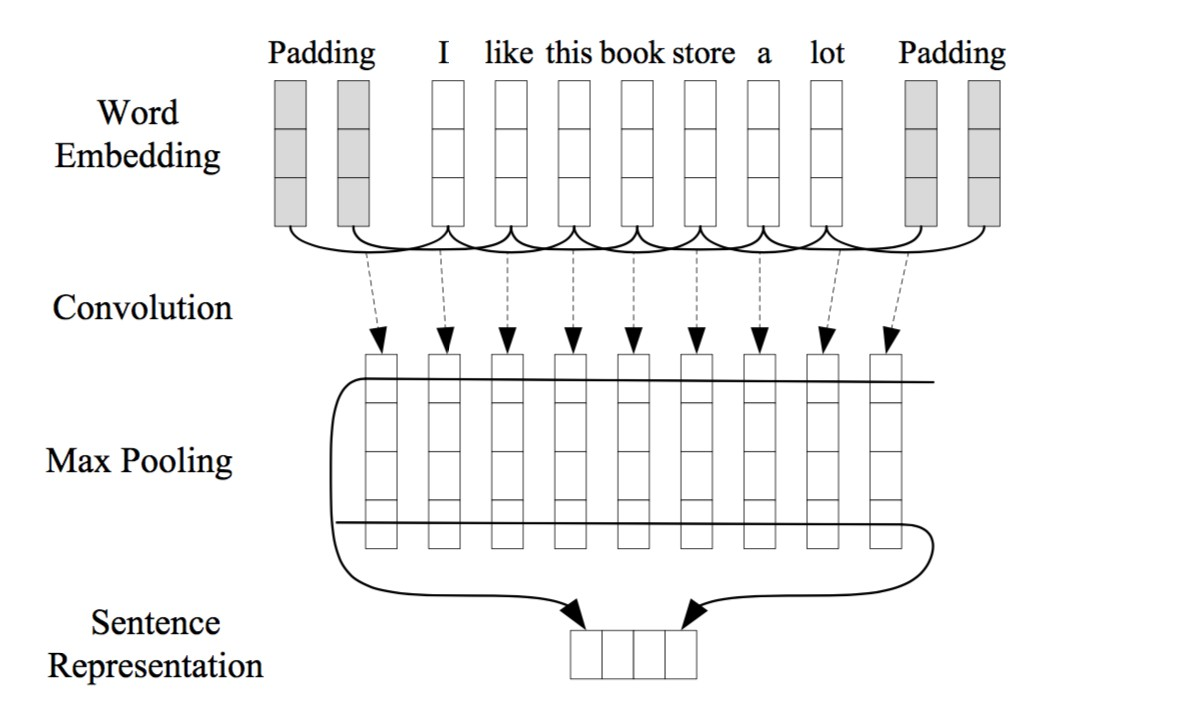
\includegraphics[width=13.25cm, height=6.75cm]{cnn}
		\caption{CNN architecture using Word2Vec vectors.}
	\end{center}
\end{figure}

If we define $\textbf{x}_i \in \mathbf{R}^k$ to be the vector representation for the $ith$ word, a sentence is the concatenation $\textbf{x}_{(1:n)} = \textbf{x}_{1} \circ \textbf{x}_{2} \circ ... \circ \textbf{x}_{n}$.  The weights of one convolution define a filter $\textbf{w} \in \mathbf{R}^{hk}$ applied to a window of $h$ words as $c_j = f(\textbf{w}^{\top} \textbf{x}_{(j:(j + h - 1))} + b)$ where $c_j$ is the $jth$ element of the response window.  Taking $\textbf{c}_i = [c_1, ..., c_{n - h + 1}]$ to be the vector response of the $ith$ convolution, max-over-time pooling is simply $\hat{c}_i = max(\textbf{c}_i)$.  We then feed all such $\hat{c}_i$ as the input vector for a fully connected feed forward DNN for binary classification.

With no hyperparameter tuning or other modifications to the original CNN the teacher and student network achieved impressive performance increases with respect to accuracy on the sentence level sentiment analysis task shown in Fig. 11.  The three different DNN models were compared against three datasets.  We see that the teacher network improves compared to the base CNN on all tasks, while the base CNN model already had very strong performance relative to the state-of-the-art.

The expert knowledge that was used for this experiment was the simple insight that a sentence which had a ``but" clause would tend to take the sentiment of the subsentence following the ``but".  For example, the sentence ``At first I was enjoying the movie but then I realized it was really bad." should be labeled as a negative review.

This logic rule is formalized as:
\begin{gather*}
\text{has-A-but-B-structure}(S) \Rightarrow \\
(\mathbf{1}(y = +) \Rightarrow \boldsymbol{\sigma}_\theta(B)_+ \land \boldsymbol{\sigma}_\theta(B)_+ \Rightarrow \mathbf{1}(y = +)),
\end{gather*}
where $\mathbf{1}(y = +)$ is an indicator function over the label of $y$ with value $1$ when $y$ is positive and $0$ otherwise.  $\boldsymbol{\sigma}_\theta(B)_+$ is the element of $\boldsymbol{\sigma}_\theta(B)$ (the prediction vector of the student network given only the subsentence $B$) which corresponds to the positive label.
\begin{figure}
	\begin{center}
		\begin{tabular}{ | l | l | l | p{3cm} |}
			\hline
			Model & SST2 & MR & CR \\ \hline
			Base CNN & 87.2 & 81.3 $\pm$ 0.1& 84.3 $\pm$ 0.2  \\
			Student CNN (p) & 88.8 & 81.6 $\pm$ 0.1 & 85.0 $\pm$ 0.3 \\
			Teacher CNN (q) & 89.3 & 81.7 $\pm$ 0.1 & 85.3 $\pm$ 0.3 \\
			\hline
		\end{tabular}
	\end{center}
	\caption{Results of the teacher and student architecture extending a base CNN model.}
\end{figure}
Assuming the rule $\text{has-A-but-B-structure}(S)$ for sentence $S$ holds we can rewrite the above formula using basic logical equivalences as:
\begin{gather}
\neg \mathbf{1}(y = +) \lor \boldsymbol{\sigma}_\theta(B)_+ \land \neg \boldsymbol{\sigma}_\theta(B)_+ \lor \mathbf{1}(y = +).
\end{gather}

Using the soft logic semantics defined in Eq. 7 the truth value of the above rule is:
\begin{gather*}
(10) = 
\begin{cases}
(1 + \boldsymbol{\sigma}_\theta(B)_+)/2, & \text{if } y = +\\
(2 - \boldsymbol{\sigma}_\theta(B)_+)/2, & \text{otherwise}
\end{cases}
\end{gather*}
Using the truth value of Eq. 10 we can construct the teacher network (Eq. 9) where $\lambda_l = 1$ in this experiment.

\section{TensorLog}
TensorLog~\cite{DBLP:journals/corr/Cohen16b} integrates probabilistic logical reasoning with DNNs using a differentiable inference procedure.  This allows for the integration of a deductive probabilistic knowledge base $\mathcal{DB}$ and theory $\mathcal{T}$ along with the set of facts derivable from $\mathcal{DB}$ using $\mathcal{T}$.

\subsection{Knowledge Base Representation}
\begin{figure}
	\begin{center}
		\begin{verbatim}
		% Theory T
			uncle(X, Y) :- child(X, Z), brother(Z, Y).
			uncle(X, Y) :- aunt(X, W), husband(W, Y).
			status(X, tired) :- child(W, X), infant(W).
			
			% Knowledge Base DB
			0.99 :: child(liam, eve).     0.7 :: infant(liam).
			0.99 :: child(dave, eve).     0.1 :: infant(dave).
			0.75 :: child(liam, bob).     0.9 :: aunt(joe, eve).
			0.9 :: husband(eve, bob).     0.9 :: brother(eve, chip).
		\end{verbatim}
	\end{center}
	\caption{Example $\mathcal{DB}$ and $\mathcal{T}$.}
\end{figure}
An example $\mathcal{DB}$ and $\mathcal{T}$ are given in Fig. 12.  All predicates have at most binary arity over the domain and there are no function symbols.  Additionally we adopt a similar notation to ProbLog where $\theta :: r$ is the probability of the binary random variable corresponding to the predicate holding in some world.  TensorLog can only model restricted Datalog programs of this form and does so using matrix representations of predicates and constants.

Constants $c \in C$ are represented using a one-hot row-vector $\textbf{u} \in \mathbf{R}^{|C|}$.  It is assumed that there is some arbitrary order on $c \in C$ corresponding to indices $[1, ..., |C|]$ which holds in all matrices and vectors.  Binary predicates are represented as a sparse matrix $\textbf{M}_r$ where $\textbf{M}_r[i, j] = \theta_{r(i, j)}$ if $r(i, j) \in \mathcal{DB}$, and 0 otherwise.  For example $\theta_{child(liam, eve)} = .75$ in the model shown in Fig. 12.  A unary predicate $q$ is represented analogously as a row-vector $\textbf{v}_q$.

For a query $\textbf{q}(a, Y)$ TensorLog will compute a response vector $\textbf{v}_Y \in \mathbf{R}^{|C|}$ where:
\begin{gather*}
\textbf{v}_{Y}[b] = p( \textbf{q}(a, b) | \mathcal{T}, \mathcal{DB}).
\end{gather*}  We will also be interested in the conditional probabilities:
\begin{gather*}
\textbf{v}_{Y|a}[b] = p( f = \textbf{q}(a, b) |f \in U_{\textbf{q}(a, Y)}, \mathcal{T}, \mathcal{DB}),
\end{gather*} where $U_{\textbf{q}(a, Y)}$ is the set of instances of $\textbf{q}(a, Y)$.  $\textbf{v}_{Y|a}$ is simply the normalized $\textbf{v}_{Y}$ which can be useful for determining which is the most likely grounding of the query variable.  An analogous computation is performed for a query $\textbf{q}(X, b)$.  

For notational purposes let $f_{\text{io}}^{r}(\textbf{u}_a) = \textbf{v}_{Y|a}$ be the function which computes the normalized response vector for query $r(a, Y)$ and $f_{\text{oi}}^{r}(\textbf{u}_b) = \textbf{v}_{X|b}$ be the function for $r(X, b)$.  Let $g_{\text{io}}^{r}$ and $g_{\text{oi}}^{r}$ be functions which return unnormalized response vectors $p( \textbf{q}(a, b) | \mathcal{T}, \mathcal{DB})$.  The subscripts io and oi correspond to the position of the unground logical variable (o) and the ground variable (i).  

\subsection{Factor Graph Construction}

\begin{figure}
	\begin{center}
		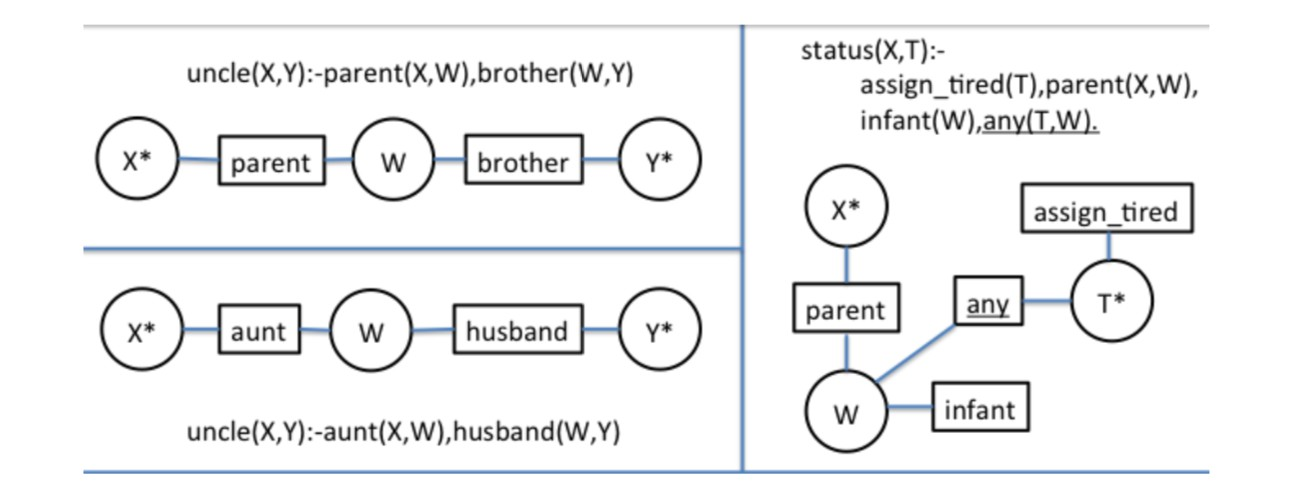
\includegraphics[width=12cm, height=5cm]{tensorlog}
		\caption{Factor graph representation of clauses.}
	\end{center}
\end{figure}
The key insight into TensorLog's differentiable inference is similar to that of Markov Logic Networks.  As in MLNs TensorLog transforms the probabilistic logical rules into a PGM and uses standard inference techniques for PGMs to compute the probability of a query.  Specifically, TensorLog transforms the knowledge base and theory into a set of factor graphs $G_r = (V_r, E_r)$ over each rule $r$ and uses belief propagation to perform inference.

One of the key advantages of TensorLog's inference method is that is space efficient compared to other representations such as MLNs.  This is because TensorLog does not explicitly ground the variables of the factor graph but represents the possible instantiations with matrices and vectors.

TensorLog introduces two special predicates to assist in the factor graph construction: \verb!any/2! which holds with probability 1 for all possible groundings (ie. has a factor matrix of all ones) and \verb!assign/1! which handles constants.  As an example, \verb!assign_tired(T)! would replace the constant \verb!tired! in \verb!status(X, tired)! as \verb!status(X, T) :- assign_tired(T)!.  The only fact in $\mathcal{DB}$ for \verb!assign_tired(T)! is \verb!assign_tired(tired)!.

TensorLog transforms clauses into a factor graph with the following construction: \\
1. For each logical variable $X$: create a node $X$\\
2. For each predicate $P$ in the body of the clause: create a factor $P$ with edges $(X, P)$ for all arguments $X$ with potentials defined by $\textbf{M}_P$\\
3. Add \verb!any/2! factors to connect the graph (if it is not fully connected).

Fig. 13 shows examples of the factor graph construction where variables which appear in the head of the clause are starred.  $G_r$ is defined over the body of a clause and will determine the probability of the head for each grounding.

$G_r$ defines a distribution over possible groundings of the variables in $r$.  Let $X_1, ..., X_m$ be the variables in $r$.  Then:
\begin{gather*}
p_{G_r}(X_1 = c_1, ..., X_m = c_m) = \frac{1}{Z} \prod_{(c_i, c_j) \in E_r} \phi_r(c_i, c_j) = \prod_{(c_i, c_j) \in E_r} \theta_{r(c_i, c_j)}.
\end{gather*}
If $r(c_i, c_j) \notin \mathcal{DB}$ any substitution $r(X_i, X_j)\{X_i / c_i, X_j / c_j\}$ will have 0 probability.

\subsection{Inference}
Given that the predicates in $\mathcal{KB} \cup \mathcal{T}$ have at most arity two, the BP algorithm for $G_r$ is relatively simple and is presented in Algorithm 4.  It is assumed that $G_r$ is a polytree (a DAG which has an underlying undirected graph that is a tree) and that there are no recursive rules in $\mathcal{T}$.
\begin{mdframed}[linewidth=.8pt]
	\begin{algorithm}[H]
		\Fn{compileMessage$(F \rightarrow X)$: }{
			
			\KwData{
				Factor $F$ representing $r(X)$ or $r(X_i, X_o)$, \\
				\hspace*{1.15cm} Random variable $X$ representing the logical variable
			}
			\KwResult{Message from $F$ to $X$: $\textbf{v}_{F, X}$\newline}
			\uIf{$F = r(X)$}{
				$\textbf{v}_{F, X} \leftarrow \textbf{v}_r$
			}
			\uElseIf{$X$ is the output variable $X_o$ of $F$}{
				$\textbf{v}_i \leftarrow \text{compileMessage}(X_i \rightarrow F)$\\
				$\textbf{v}_{F, X} \leftarrow \textbf{v}_i \textbf{M}_r$
			}
			\ElseIf{$X$ is the input variable $X_i$ of $F$}{
				$\textbf{v}_o \leftarrow \text{compileMessage}(X_o \rightarrow F)$\\
				$\textbf{v}_{F, X} \leftarrow \textbf{v}_o \textbf{M}_{r}^{\top}$
			}
			\textbf{return} $\textbf{v}_{F, X}$
		}
	\end{algorithm}
	
	\begin{algorithm}[H]
		\Fn{compileMessage$(X \rightarrow F)$: }{
			
			\KwData{
				Random variable $X$ representing the logical variable, \\
				\hspace*{1.15cm} Factor $F$ representing $r(X)$ or $r(X_i, X_o)$
			}
			\KwResult{Message from $X$ to $F$: $\textbf{v}_{X, F}$\newline}
			
			\uIf{$X$ is the given variable to the query}{
				$\textbf{v}_{X, F} \leftarrow \textbf{u}_c$ // return the one-hot vector
			}
			// if the only factor which has $X$ as an argument is $F$:\\
			\uElseIf{$\eta(X) = \{F\}$}{
				$\textbf{v}_{X, F} \leftarrow \textbf{1}$  // return a vector of all 1's
			}
			\Else{
				// loop over all $k$ of $X$'s neighbor literals $F_i$ except $F$\\
				\ForEach{$F_i \in \eta(X)\setminus F$}{
					$\textbf{v}_i \leftarrow \text{compileMessage}(F_i \rightarrow X)$
				}
				$\textbf{v}_{X, F} \leftarrow \textbf{v}_1 \circ ... \circ  \textbf{v}_k$ // $\circ$ is the element-wise product
			}
			\textbf{return} $\textbf{v}_{X, F}$
		}
		\caption{TensorLog Belief Propagation}
	\end{algorithm}
\end{mdframed}

We will first consider the case where $\mathcal{T}$ has a single rule to illustrate the computation procedure.  Consider the rule: 
\begin{verbatim}
                   uncle(X, Y) :- parent(X, W), brother(W, Y).
\end{verbatim}
We construct $G_{uncle}$ as shown in Fig. (?).  Assume that we are interested in the query \verb!uncle(c, Y)! for some $c \in C$.  This corresponds to the function $g_{io}^{uncle}(\textbf{u}_c)$.  Thus we will perform BP over $G_{uncle}$ conditioned on $X = c$.  This corresponds to the following linear transformation:
\begin{gather*}
(\textbf{u}_c \textbf{M}_{parent})\textbf{M}_{brother}.
\end{gather*}
Recall that $\textbf{u}_c$ is a one-hot vector which encodes the position of the constant $c \in C$.  Then $\textbf{v}_W = \textbf{u}_c \textbf{M}_{parent}$ is a vector where $\textbf{v}_W[c'] = \theta_{parent(c, c')}$.  Finally $\textbf{v}_Y = \textbf{v}_W \textbf{M}_{brother}$ computes the marginal probability for $Y$ which is exactly what BP does in the message passing steps.

BP in $G_r$ corresponds to simple linear transformations of the probability vector representations over $\mathcal{KB}$.  We can now generalize to the non-trivial case where $\mathcal{T}$ is arbitrarily large.  In the case where some predicate is defined in multiple rules we simply return the sum of the response vectors for the individual definitions.  For example, $g_{io}^{\verb!uncle!}(\textbf{u}_c) = g_{io}^{\verb!uncle!_1}(\textbf{u}_c) + g_{io}^{\verb!uncle!_2}(\textbf{u}_c)$ where $\verb!uncle!_i$ is the $ith$ definition for the predicate.  If a predicate $r$ is defined by some $r' \in \mathcal{T}$ (as opposed to some $r' \in \mathcal{DB}$) we replace $\textbf{v}_{F, X} \leftarrow \textbf{v}_i \textbf{M}_r$ with $\textbf{v}_{F, X} \leftarrow g_{io}^{r'}(\textbf{v}_i)$ in compileMessage($F \rightarrow X$).

\subsection{Learning}
In contrast to PRISM parameter learning, TensorLog will learn the parameters of the matrices and vectors using standard gradient approaches for DNNs.  Specifically TensorLog optimizes the cross-entropy loss over the prediction vector returned by $g_{io}^{\textbf{q}}$ which is normalized using a softmax activation function.

Returning again to the query \verb!uncle(c, Y)! assume that we had a training set consisting of ground facts \verb!uncle(x, y)! for some $x, y \in C$.  We would learn the parameters of $\mathcal{DB}$ by performing inference: $g_{io}^{uncle}(\textbf{u}_x) = \textbf{v}_Y$ and then computing the loss as:
\begin{gather*}
\mathcal{L}_{cross-entropy}(\textbf{u}_y, softmax(g_{io}^{uncle}(\textbf{u}_x))).
\end{gather*}
In general the ground truth vector need not be one-hot and could represent a probability distribution as well.  We then use the SGD algorithm along with backpropagation to update the parameters of $\mathcal{DB}$.

\section{Discussion}
The recent approaches for integrating logical reasoning in deep neural networks discussed in this report provide interesting new perspectives in the probabilistic logical inference problem.  We have seen that many of the well-established formalisms in the SRL literature have had great influence on the design and implementation of these systems.

The teacher/student network which we first discussed provides a prototypical logical DNN which is constructed by engineering the objective function.  It may be interesting to see how modifying this objective function would change the network behavior.  Another extension would be to integrate a different continuous logic as the logical component.  Finally, it is worth investigating if integrating logic biases in the network itself provides any tangible benefits compared to simple feature engineering (as a preprocessing step).  It may be the case that a network which learns certain logic rules could then be applied to a different problem domain while retaining these learned relationships.  This transfer learning problem may yield interesting results.

While Hu et al.'s teacher/student network is generally applicable for regularization in any DNN, TensorLog presents the possibility of a new paradigm of deep probabilistic logic programming.  The exact domains which may benefit from this tight integration of logical inference and DNNs is not yet clear.  Recently the idea of ``differentiable programming" has gained momentum in the deep learning community.  The general idea is that deep learning architectures are constructed from well known building blocks such as embedding layers, CNNs, etc.  A deductive reasoning unit such as TensorLog (and beyond) could provide a high level of expressibility for differentiable programming.  It is an interesting question to consider the role which these logical deep learning systems may play in the larger context of deep learning in the future.

One shortcoming of TensorLog is that the logical language is heavily restricted compared to Prolog's semantics.  A fairly obvious extension would be to generalize the BP procedure to handle predicates with arbitrary arity.  It seems that this should be possible by considering probability tensors instead of flat matrices.  For example, to represent a ternary predicate we would use some tensor $T$ where:
\begin{gather*}
T[i, j, k] = \theta_{r(i, j, k)}.
\end{gather*}
It is not immediately clear if this extension would still reduce to the BP algorithm over the constructed factor graphs.  Expanding the class of first-order logic which can be integrated in DNNs will be critical for the expressive power of these systems.

Earlier in the report we considered how word embeddings revolutionized NLP by giving a semantic dense vector representation for the features.  Given that the representation of logical constants in TensorLog is as one-hot vectors there may be an analogous way to train a dense feature representation over the domain $C$.  Beyond TensorLog, this idea of dense vector representations may be applicable for logical reasoning in general.  We could train a DNN on a logical learning task where the one-hot vectors are some representation of the logical knowledge base.  The learned dense vectors could then be used in a different learning task.

\subsection{Conclusion}
This report introduced a variety approaches and systems for combining logical and probabilistic systems.  The systems which were presented for combining probabilistic logic and deep neural networks provide an important foundation for future methods in this field.  While these approaches are promising, the goal of combining logic and deep learning remains an open question in general.  Hopefully this report has highlighted some of the most interesting and exciting aspects of this emerging research area.

\bibliographystyle{unsrt}
\bibliography{rpe}
\end{document}

